
\begin{figure}[ht]
\centering
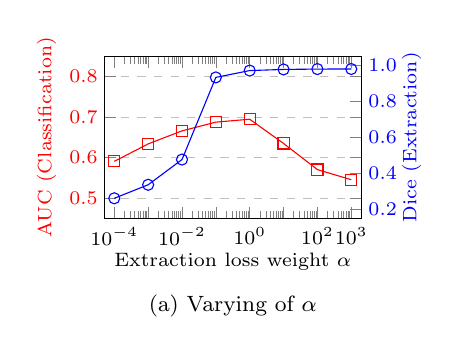
\begin{tikzpicture}
\begin{semilogxaxis}[
    title = {(a) Varying of $\alpha$},
    outer sep=0,
    width=0.4\columnwidth,
    height=0.3\columnwidth,
    xlabel={\textcolor{black}{Extraction loss weight $\alpha$}},
    x label style={at={(axis description cs:0.5,-0.16)},anchor=north},
    ylabel={\textcolor{red}{AUC (Classification)}},
    ylabel style={at={(axis description cs:-0.15,0.5)},anchor=south},
    yticklabel style={text=red,xshift=1pt},
    xmin=0.00005, xmax=2000,
    ymin=0.45, ymax=0.85, % 根据数据1调整
    xtick={0.0001, 0.001, 0.01, 0.1, 1, 10, 100, 1000},
    xticklabels={$10^{-4}$, \empty, $10^{-2}$, \empty, $10^{0}$, \empty, $10^{2}$, $10^{3}$},
    ytick={0.5, 0.6, 0.7, 0.8},
    yticklabels={0.5, 0.6, 0.7, 0.8},
    ymajorgrids=true,
    grid style=dashed,
    tick label style={font=\scriptsize},
    label style={font=\scriptsize, text=red},
    title style={font=\footnotesize, align=right, yshift=-0.3\columnwidth},
]

% 数据1
\addplot[
    color=red,
    mark=square,
    ]
    coordinates {
    (0.0001, 0.5909)
    (0.001, 0.6340)
    (0.01, 0.6662)
    (0.1, 0.6878)
    (1, 0.6950)
    (10, 0.6351)
    (100, 0.5706)
    (1000, 0.5455)
    };

\end{semilogxaxis}

\begin{semilogxaxis}[
    axis y line*=right,
    axis x line=none,
    width=0.4\columnwidth,
    height=0.3\columnwidth,
    ylabel={\textcolor{blue}{Dice (Extraction)}},
    ylabel style={at={(axis description cs:1.27,0.5)},anchor=south},
    yticklabel style={text=blue,xshift=-1pt},
    xmin=0.00005, xmax=2000,
    ymin=0.15, ymax=1.05, % 根据数据2调整
    ytick={0.2, 0.4, 0.6, 0.8, 1.0},
    yticklabels={0.2, 0.4, 0.6, 0.8, 1.0},
    tick label style={font=\scriptsize},
    label style={font=\scriptsize, text=blue},
]

% 数据2
\addplot[
    color=blue,
    mark=o,
    ]
    coordinates {
    (0.0001, 0.2617)
    (0.001, 0.3368)
    (0.01, 0.4770)
    (0.1, 0.9337)
    (1, 0.9717)
    (10, 0.9780)
    (100, 0.9800)
    (1000, 0.9805)
    };

\end{semilogxaxis}
\end{tikzpicture}
\label{fig:vary a}
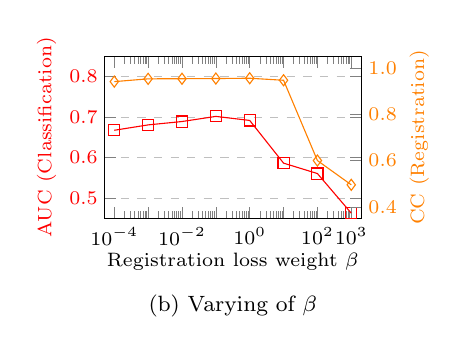
\begin{tikzpicture}
\begin{semilogxaxis}[
    title = {(b) Varying of $\beta$},
    outer sep=0,
    width=0.4\columnwidth,
    height=0.3\columnwidth,
    xlabel={\textcolor{black}{Registration loss weight $\beta$}},
    x label style={at={(axis description cs:0.5,-0.16)},anchor=north},
    ylabel={\textcolor{red}{AUC (Classification)}},
    ylabel style={at={(axis description cs:-0.15,0.5)},anchor=south},
    yticklabel style={text=red,xshift=1pt},
    xmin=0.00005, xmax=2000,
    ymin=0.45, ymax=0.85, % 根据数据1调整
    xtick={0.0001, 0.001, 0.01, 0.1, 1, 10, 100, 1000},
    xticklabels={$10^{-4}$, \empty, $10^{-2}$, \empty, $10^{0}$, \empty, $10^{2}$, $10^{3}$},
    ytick={0.5, 0.6, 0.7, 0.8},
    yticklabels={0.5, 0.6, 0.7, 0.8},
    ymajorgrids=true,
    grid style=dashed,
    tick label style={font=\scriptsize},
    label style={font=\scriptsize, text=red},
    title style={font=\footnotesize, align=right, yshift=-0.3\columnwidth},
]

% 数据1
\addplot[
    color=red,
    mark=square,
    ]
    coordinates {
    (0.0001, 0.6677)
    (0.001, 0.6810)
    (0.01, 0.6893)
    (0.1, 0.7020)
    (1, 0.6920)
    (10, 0.5865)
    (100, 0.5608)
    (1000, 0.4629)
    };

\end{semilogxaxis}
\begin{semilogxaxis}[
    axis y line*=right,
    axis x line=none,
    width=0.4\columnwidth,
    height=0.3\columnwidth,
    ylabel={\textcolor{orange}{CC (Registration)}},
    ylabel style={at={(axis description cs:1.30,0.5)},anchor=south},
    yticklabel style={text=orange,xshift=-1pt},
    xmin=0.00005, xmax=2000,
    ymin=0.35, ymax=1.05, % 根据数据2调整
    ytick={0.4, 0.6, 0.8, 1.0},
    yticklabels={0.4, 0.6, 0.8, 1.0},
    tick label style={font=\scriptsize},
    label style={font=\scriptsize, text=blue},
]

% 数据2
\addplot[
    color=orange,
    mark=diamond,
    ]
    coordinates {
    (0.0001, 0.9413)
    (0.001, 0.9534)
    (0.01, 0.9539)
    (0.1, 0.9547)
    (1, 0.9560)
    (10, 0.9472)
    (100, 0.6000)
    (1000, 0.4951)
    };

\end{semilogxaxis}
\end{tikzpicture}
\label{fig:vary b}
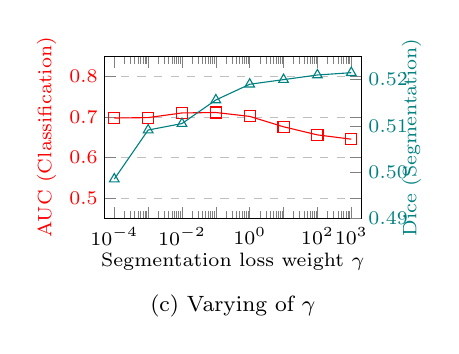
\begin{tikzpicture}
\begin{semilogxaxis}[
    title = {(c) Varying of $\gamma$},
    outer sep=0,
    width=0.4\columnwidth,
    height=0.3\columnwidth,
    xlabel={\textcolor{black}{Segmentation loss weight $\gamma$}},
    x label style={at={(axis description cs:0.5,-0.16)},anchor=north},
    ylabel={\textcolor{red}{AUC (Classification)}},
    ylabel style={at={(axis description cs:-0.15,0.5)},anchor=south},
    yticklabel style={text=red,xshift=1pt},
    xmin=0.00005, xmax=2000,
    ymin=0.45, ymax=0.85, % 根据数据1调整
    xtick={0.0001, 0.001, 0.01, 0.1, 1, 10, 100, 1000},
    xticklabels={$10^{-4}$, \empty, $10^{-2}$, \empty, $10^{0}$, \empty, $10^{2}$, $10^{3}$},
    ytick={0.5, 0.6, 0.7, 0.8},
    yticklabels={0.5, 0.6, 0.7, 0.8},
    ymajorgrids=true,
    grid style=dashed,
    tick label style={font=\scriptsize},
    label style={font=\scriptsize, text=red},
    title style={font=\footnotesize, align=right, yshift=-0.3\columnwidth},
]

% 数据1
\addplot[
    color=red,
    mark=square,
    ]
    coordinates {
    (0.0001, 0.6980)
    (0.001, 0.6990)
    (0.01, 0.7105)
    (0.1, 0.7116)
    (1, 0.7020)
    (10, 0.6763)
    (100, 0.6563)
    (1000, 0.6457)
    };

\end{semilogxaxis}

\begin{semilogxaxis}[
    axis y line*=right,
    axis x line=none,
    width=0.4\columnwidth,
    height=0.3\columnwidth,
    ylabel={\textcolor{teal}{Dice (Segmentation)}},
    ylabel style={at={(axis description cs:1.27,0.5)},anchor=south},
    yticklabel style={text=teal,xshift=-1pt},
    xmin=0.00005, xmax=2000,
    ymin=0.49, ymax=0.525, % 根据数据2调整
    ytick={0.49, 0.50, 0.51, 0.52},
    yticklabels={0.49, 0.50, 0.51, 0.52},
    tick label style={font=\scriptsize},
    label style={font=\scriptsize, text=blue},
]

% 数据2
\addplot[
    color=teal,
    mark=triangle,
    ]
    coordinates {
    (0.0001, 0.4985)
    (0.001, 0.5091)
    (0.01, 0.5105)
    (0.1, 0.5156)
    (1, 0.5190)
    (10, 0.5200)
    (100, 0.5210)
    (1000,0.5215)
    };

\end{semilogxaxis}
\label{fig:vary-c}
\end{tikzpicture}
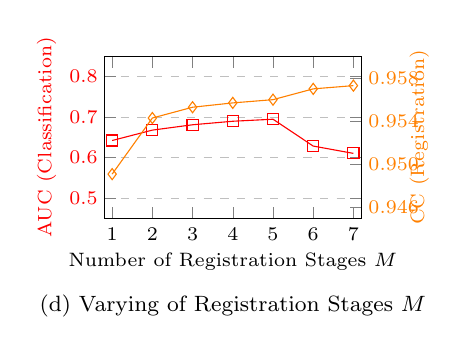
\begin{tikzpicture}
\begin{axis}[
    title = {(d) Varying of Registration Stages $M$},
    outer sep=0,
    width=0.4\columnwidth,
    height=0.3\columnwidth,
    xlabel={\textcolor{black}{Number of Registration Stages $M$}},
    x label style={at={(axis description cs:0.5,-0.16)},anchor=north},
    ylabel={\textcolor{red}{AUC (Classification)}},
    ylabel style={at={(axis description cs:-0.15,0.5)},anchor=south},
    yticklabel style={text=red,xshift=1pt},
    xmin=0.8, xmax=7.2, % 根据新数据调整
    ymin=0.45, ymax=0.85, % 根据数据1调整
    xtick={1, 2, 3, 4, 5, 6, 7},
    xticklabels={1, 2, 3, 4, 5, 6, 7},
    ytick={0.5, 0.6, 0.7, 0.8},
    yticklabels={0.5, 0.6, 0.7, 0.8},
    ymajorgrids=true,
    grid style=dashed,
    tick label style={font=\scriptsize},
    label style={font=\scriptsize, text=red},
    title style={font=\footnotesize, align=right, yshift=-0.3\columnwidth},
]

% 新的数据1
\addplot[
    color=red,
    mark=square,
    ]
    coordinates {
    (1, 0.6424)
    (2, 0.6681)
    (3, 0.6813)
    (4, 0.6900)
    (5, 0.6950)
    (6, 0.6287)
    (7, 0.6106)
    };

\end{axis}

\begin{axis}[
    axis y line*=right,
    axis x line=none,
    width=0.4\columnwidth,
    height=0.3\columnwidth,
    ylabel={\textcolor{orange}{CC (Registration)}},
    ylabel style={at={(axis description cs:1.30,0.5)},anchor=south},
    yticklabel style={text=orange,xshift=-1pt},
    xmin=0.8, xmax=7.2, % 根据新数据调整
    ymin=0.945, ymax=0.960, % 根据需要调整
    ytick={0.946, 0.950, 0.954, 0.958},
    yticklabels={0.946, 0.950, 0.954, 0.958},
    tick label style={font=\scriptsize},
    label style={font=\scriptsize, text=blue},
]

% 新的数据2
\addplot[
    color=orange,
    mark=diamond,
    ]
    coordinates {
    (1, 0.9491)
    (2, 0.9543)
    (3, 0.9553)
    (4, 0.9557)
    (5, 0.9560)
    (6, 0.9570)
    (7, 0.9573)
    };

\end{axis}
\end{tikzpicture}
    \vspace{-6pt}
    \caption{Effect of varying the extraction loss weight $\alpha$, registration loss weight $\beta$, segmentation loss weight $\gamma$ and registration stages $M$.}
    \label{fig:stage dice}
    \vspace{-11pt}
\end{figure}

